\subsection{Erweiterungen des Integralbegriffs}

\subsubsection{Uneigentliche Integrale}

\textbf{Ziel:} Die Erweiterung des Integralbegriffs auf Integranden, die 
möglicherweise nicht beschränkt sind, beziehungsweise auf Integrationsintervalle, 
die nicht beschränkt sind.

\begin{enumerate}
	\item Eine Intervallgrenze ist unendlich.
\end{enumerate}

\begin{Definition}{
	Sei $f : [a,b] \rightarrow \mathbb{R}$ auf jedem Intervall $[a,b] \subsetneq
	[a, \infty)$ Riemann-integrierbar. \\
	Wir sagen $f$ ist auf $[a, \infty)$ \emph{uneigentlich integrierbar} 
	beziehungsweise $\int_a^{\infty} f \dd{x}$ existiert, sofern der 
	folgende Grenzwert existiert:
	\begin{align*}
		\int_a^{\infty} f \dd{x} := \lim\limits_{b \rightarrow \infty}
			{\int_a^b f \dd{x}}
	\end{align*}
	Analog definiert man $\int_{-\infty}^b f \dd{x}$ für $f: (-\infty, b)
	 \rightarrow \mathbb{R}$.
}\end{Definition}

\begin{Beispiel}{
	\begin{align*}
		\int_1^{\infty} \frac{\mathrm{d}x}{x^s} = & \frac{1}{s-1} \text{für s > 1 }
	\end{align*}
	\begin{figure}
		\centering
		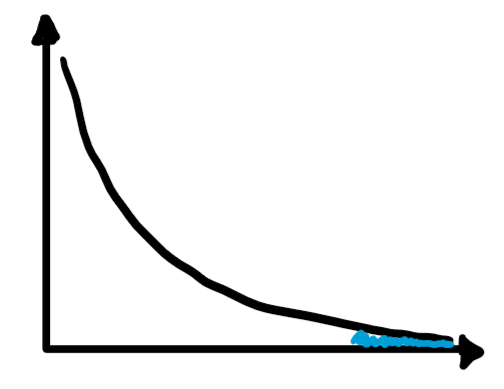
\includegraphics[scale=0.3]{Skizzen/plot_bsp_uneigentlichesIntegral}
	\end{figure}
	\todo{Caption fehlt}
	Denn: für $b > 1$ gilt:
	\begin{align*}
		\int_a^b \frac{\mathrm{dx}}{x^s} \dd{x} = & \int_a^b x^{-s} \dd{x}
		  = \left.\frac{x^{-s+1}}{-s+1} \right\vert_a^b \\
		   = & \frac{\left( b^{-s+1} - a^{-s+1}\right)}{-s+1} \overset{a = 1}{=}
		  \frac{1}{s-1}\left(1-b^{-s+1}\right) 
		  \overset{b \rightarrow \infty}{\longrightarrow}
		  \frac{1}{s-1}
	\end{align*}
	Hingegen ist $\frac{1}{x^s}$ nicht unendlich integrierbar über $[1, \infty)$,
	falls $s \leq 1$.\\
	Für $s=1$ folgt das wie folgt:
	\begin{align*}
		\int_1^b \frac{\mathrm{dx}}{x} = \left. \ln(x) \right\vert_1^b 
		= \ln b \overset{b \rightarrow \infty}{\longrightarrow} \infty
	\end{align*}
}\end{Beispiel}

\begin{enumerate}[resume]
	\item Der Integrand ist an einer Invervallgrenze kritisch (also beispielsweise 
	unbeschränkt).
\end{enumerate}

\begin{Definition}{
	Sei $f: (a, b] \rightarrow \mathbb{R}$ für jedes $ \epsilon \in (0, b-a)$ 
	über $[a + \epsilon, b]$ Riemann-integrierbar. Dann sagen wir, dass $f$ 
	über $(a,b]$ \emph{uneigentlich integrierbar} ist beziehungsweise dass 
	$\int_a^b f \dd{x}$ existiert, sofern folgender Grenzwert existiert:
	\begin{align*}
		\int_a^b f \dd{x} := \lim\limits_{\epsilon \rightarrow 0}
		{\int_{a + \epsilon}^b f \dd{x}}
	\end{align*}
	Analog bestimmt man $\int_a^b f \dd{x}$, falls b kritisch ist.
}\end{Definition}

\begin{Beispiel}{\label{vl_13_bsp_2}
	\begin{align*}
		\int_0^1 \frac{\mathrm{dx}}{x^s} \text{ existiert für } s < 1
	\end{align*}
	für $\epsilon > 0$ gilt:
	\begin{align*}
		\int_{\epsilon}^1 \frac{\mathrm{dx}}{x^s} = \int_{\epsilon}^1 x^{-s} \dd{x} 
		= \left. \frac{x^{-s+1}}{-s+1} \right\vert_{\epsilon}^1 
		= \frac{1}{1-s} (1- \epsilon^{1-s}) \overset{\epsilon \rightarrow 0}
		{\longrightarrow}\frac{1}{1-s}
	\end{align*}
}\end{Beispiel}


\begin{enumerate}[resume]
	\item Beide Integrationsgerenzen sind kritisch
\end{enumerate}

\begin{Definition}{
	Sei $f:(a,b) \rightarrow \mathbb{R}$ mit $a \in \mathbb{R} \cup \{ \infty\}$ 
	und $b \in \mathbb{R} \cup \{-\infty\}$ für alle $\alpha \in (a,b)$ und 
	$\beta \in (\alpha, b)$ Riemann-integrierbar über $[\alpha, \beta]$.
	Dann definiert man das \emph{uneigentliche Integral} von f über $[a,b]$ und 
	sagt $\int_a^b f \dd{x}$ existiert, sofern folgender Grenzwert existiert:
	\begin{align*}
		\int_a^b f \dd{x} = \lim\limits_{\epsilon \rightarrow 0}{\int_{a + \epsilon}
		^c f \dd{x}} + \lim\limits_{\delta \rightarrow 0}{\int_c ^{b - \delta} f 
		\dd{x}} \text{ wobei } c \in (a,b) \text{ sei}
	\end{align*}
}\end{Definition}


\begin{Bemerkung}{
	\begin{itemize}
		\item[ ]
		\item Die obige Definition ist unabhängig von der konkreten Wahl der 
		Zwischenstelle $c$
		\item Ist $f \in \riemann a b$ so stimmt das Riemann-Integral von $f$ über 
		$[a,b]$ mit dem uneigentlichen Integral überein.
	\end{itemize}
}\end{Bemerkung}

\begin{Satz}{
	Sei $f : [1, \infty) \rightarrow \mathbb{R}$ eine monoton fallende 
	positive Funktion. 
	Dann gilt:
	\begin{align*}
		\sum_{n = 1}^{\infty} f(n) \text{ konvergiert} \Leftrightarrow 
		\int_1^{\infty} f \dd{x} \text{ existiert}
	\end{align*}
	\begin{figure}
	\centering
		\caption{Monoton fallende positive Funktion}
		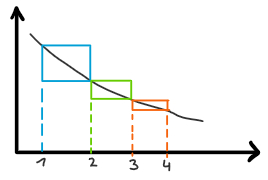
\includegraphics[scale=0.9]{Skizzen/plot_monotone_fkt_integral}
	\end{figure}
}\end{Satz}

\begin{proof}
	$\Rightarrow$ Wir setzen $g(x) = f( \lfloor x \rfloor )$ \\
	Dann gilt:
	\begin{itemize}
		\item $g(x) \geq f(x)$ $(x \in [1, \infty])$
		\item $g \in \riemann 1 b$ für alle $ b > a$
	\end{itemize}
	\begin{align*}
		\int_1^b f \dd{x} \leq \int_1^b g \dd{x} \leq \sum_{n = 1}^{\lceil b \rceil}
		f(n) \leq \sum_{n=1}^{\infty} f(n) < \infty 
	\end{align*}
	$\Leftarrow$ Sei $ h(x) = f(\lceil x \rceil )$ Dann gilt:
	\begin{itemize}
		\item $h \in \riemann 1 b $ für $b >a$
		\item $h(x) \leq f(x) $ $ (x \in [1, \infty)) $
	\end{itemize}
	Damit gilt:
	\begin{align*}
		\sum_{n = 1}^{\lceil b \rceil }f(n) = f(1) + 
		\int_1^{\lceil b \rceil}h(x) \dd{x} 
		\leq f(1) + \int_1^{\lceil b \rceil} f \dd{x} < \infty
	\end{align*}
\end{proof}

\textbf{Anwendung:} $\sum_{n=1}^{\infty}\frac{1}{n^s}$ konvergiert für jedes $s > 1$

\begin{Bemerkung}[Gauß-Klammer]{
	\begin{itemize}
		\item[ ]
		\item für $x \in \mathbb{R}$ bezeichnet $\lfloor x \rfloor$ die größte ganze 
		Zahl kleiner gleich $x$ und $\lceil x \rceil$ die kleinste ganze Zahl größer 
		gleich $x$
	\end{itemize}
}\end{Bemerkung}

\begin{itemize}
	\item Die \emph{Gamma-Funktion} 
	\begin{align*}
		\Gamma : (0, \infty) \rightarrow & \mathbb{R} \\
		x \mapsto & \int_0^{\infty} t^{x-1}exp(-t) \dd{t} \\
		\Gamma(n) = & \int_0^1 (- \log x)^{n-1} \dd{x}
	\end{align*}
	Die $\Gamma$-Funktion ist wohldefiniert. Da 
	\begin{align*}
	t^{x-1}exp(-t) \overset{t \rightarrow \infty}{\longrightarrow} 0 
	\end{align*}			
	existiert ein $t_0 \in (0, \infty)$ mit:
	\begin{align*}
		t^{x-1}exp(-t) < \frac{1}{t^2} \text{ }( t \geq t_0)
	\end{align*}
\end{itemize}
Damit gilt:
\begin{itemize}
	\item $\int_{t_0}^{\infty} t^{x-1}exp(-t) \dd{t} \leq \int_{t_0}^{\infty}
	\frac{\dd{t}}{t^2} < \infty$
	\item $\int_0^{t_0} t^{x-1}exp(-t) \dd{t} \leq \int_0^{t_0} t^{x-1} \dd{t} < 
	\infty$ (siehe Beispiel~\ref{vl_13_bsp_2})
\end{itemize}

\begin{Satz}[Funktionsgleichung der $\Gamma$-Funktion]{
	Für $x > 0 $ gilt:
	\begin{align*}
		\Gamma (x +1) = x \cdot \Gamma(x)
	\end{align*}
}\end{Satz}

\begin{Bemerkung}{
	\begin{itemize}
		\item[ ]
		\item $\Gamma(1) = 1$ (einfach nachrechnen)
		\item $\Gamma(2) = 2 \cdot \Gamma(2) = 2$ 
		\item[ ] und so weiter. Wir sehen: 
		\begin{align*}
			\Gamma(n+1) = n !
		\end{align*}
	\end{itemize}
}\end{Bemerkung}

\begin{proof}
	Sei $\epsilon > 0, R > \epsilon$ Dann gilt:
	\begin{align*}
		\int_{\epsilon}^{R}t^{x-1} exp(-t) \dd{t}  = & 
			\left. -t^{x-1} \cdot exp(-t) \right\vert_{\epsilon}^R 
			+ \int_{\epsilon}^{R}(x-1)t^{x-2}exp(-t) \dd{t} \\
			\text{ Für } x > 1 \text{ gilt daher }
			\Gamma(x) = &  (x-1) \Gamma(x-1)
	\end{align*}
\end{proof}
\todo{ Bemerkung statt x -1 -> x+1 ? }

\subsubsection{Integrale über komplexwertige Funktionen}

\begin{Definition}{
	Sei $f: [a,b] \rightarrow \mathbb{C}$. Dann heißt $f$ auf $[a,b]$ 
	\emph{Riemann-integrierbar}, falls $Re(f)$ und $Im(f)$ (Realteil beziehungsweise 
	Imaginärteil von f) Riemann-integrierbar sind über $[a,b]$. In diesem Falle 
	definieren wir:
	\begin{align*}
		\int_a^b f \dd{x} = \int_a^b Re(f) \dd{x} + i \int_a^b Im(f) \dd{x}
	\end{align*}
}\end{Definition}

\begin{Satz}{
	Seien $f, f_1, f_2: [a,b] \rightarrow \mathbb{C}$ Riemann-integrierbar über 
	$[a,b]$, dann gilt:
	\renewcommand{\labelenumi}{\alph{enumi})}
	\begin{enumerate}
		\item Für $c \in \mathbb{C}$ ist $c \cdot f$ Riemann-integrierbar über 
		$[a,b]$ sowie $f_1 + f_2$ und es gilt:
		\begin{align*}
			\int_a^b f_1 + f_2 \dd{x} = &\int_a^b f_1 \dd{x} + \int_a^b f_2 \dd{x}\\
			\int_a^b c \cdot f \dd{x} = & c \cdot \int_a^b f \dd{x} 
		\end{align*}
		\item Ist $ c \in (a,b)$, so ist $f$ über $[a,c]$ und über $[c,b]$ 
		integrierbar und es gilt:
		\begin{align*}
			\int_a^b f \dd{x} = \int_a^c f \dd{x} + \int_c^b f \dd{x}
		\end{align*}
		\item $f_1 \cdot f_2$ ist integrierbar über $[a,b]$
		\item $\overline{f}$ ist integrierbar über $[a,b]$
		\item $\abs{f}$ ist integrierbar und es gilt:
		\begin{align*}
			\abs{\int_a^b f \dd{x} } \leq \int_a^b \abs{f} \dd{x}
		\end{align*}
	\end{enumerate}
	\todo{Punkt f fehlt oben ?}
}\end{Satz}

\begin{proof}
	a)-d) folgen sofort aus den Eigenschaften des Integrals über reellwertige 
	Funktion
	\begin{itemize}
		\item[e)] $\abs{f} = \sqrt{f \cdot \overline{f}}$ ist integrierbar, 
		auf Grund von c), d) und Satz~\ref{vl_11_satz24} 
		\item[f)] Wähle $\varphi \in [0, 2\pi)$, so dass:
		\begin{align*}
			exp(i \varphi) \cdot \int_a^b f \dd{x} \in \mathbb{R} \text{ Dann gilt:} \\
			\abs{\int_a^b f\dd{x} } = & \abs{exp(i \varphi) \cdot \int_a^b f \dd{x}} \\
			 = & \abs{ \int_a^b exp(i \varphi) \cdot f \dd{x}} = \abs{ \int_a^b   
			Re(exp(i \varphi) f) \dd{x}} \\
			 \leq & \int_a^b \abs{Re(exp(i \varphi) f} \dd{x}
			\leq \int_a^b \abs{ exp(i \varphi) f } \dd{x} \\
			= & \int_a^b \abs{f} \dd{x}
		\end{align*}
	\end{itemize}
\end{proof}

\begin{Bemerkung}{
	$\abs{exp(i \varphi)} > 0$
}\end{Bemerkung}